\begin{minipage}[t]{200mm}
\fcolorbox{black}{white}{
\begin{minipage}[b]{0.35\linewidth}
\Huge \textbf{UNF NEWS} \\
\Large -- I før-fremtid har katte det godt!
\end{minipage}
\begin{minipage}[b]{0.4\linewidth}
\Large Søndag 14.07.2012 \\
\normalsize Redigeret i \LaTeX\ af \\ SOM, MGS, WIL

\end{minipage}
}
\end{minipage}
\hfill
\begin{minipage}[t]{200mm}
\fcolorbox{black}{white}{
\begin{minipage}[b]{0.35\linewidth}
\Huge \textbf{UNF NEWS} \\
\Large -- I før-fremtid har katte det godt!
\end{minipage}
\begin{minipage}[b]{0.4\linewidth}
\Large Søndag 14.07.2012 \\
\normalsize Redigeret i \LaTeX\ af \\ SOM, MGS, WIL

\end{minipage}
}
\end{minipage}
\end{minipage}

\begin{minipage}[b]{1.95\textwidth}
\begin{minipage}[t]{0.23\linewidth}
\vspace{3mm}
\section*{Parringsritual -- Ewok}

%\begin{center}
%$\quad$\hspace{4cm}
%
\includegraphics[width=0.8\linewidth]{Ewok.jpg}
%\end{center}
\end{minipage}
%\hspace{2mm}
\hfill
\begin{minipage}[t]{0.73\linewidth}
\begin{minipage}[t]{0.64\linewidth}
\vspace{3mm}
\section*{IMO 2012 opgave 3}
Løgnerens gætteleg er et spil for to spillere A og B. Spillets regler bygger på to positive
heltal $k$ og $n$ som begge spillere kender. Ved spillets start vælger A hele tal $x$ og $N$, så $1 \le x \le N$. Spiller A holder $x$ hemmelig, men fortæller sandfærdigt spiller B hvad $N$ er. Derefter prøver spiller B at få information om $x$ ved at stille spiller A spørgsmål på følgende måde: Hvert spørgsmål består af at B vælger en vilkårlig mængde $S$ af positive heltal (evt. en som han allerede har valgt før) og spørger A om $x$ tilhører $S$. Spiller B må stille så mange spørgsmål han vil. Efter hvert spørgsmål skal spiller A omgående svare ja eller nej, men hun må lyve så mange gange hun har lyst til. Den eneste begrænsning er at der blandt vilkårlige $k + 1$ på hinanden følgende svar skal være mindst et svar som er sandt. Efter at B har stillet så mange spørgsmål som han vil, skal han angive en mængde $X$ med højst $n$ positive heltal. Hvis $x$ tilhører $X$, vinder B; og hvis ikke, taber han. Vis at:
\begin{enumerate}
\item[0.] Vis at hvis $k=1$ og $n=2$, har B en vindende strategi.
\item[1.] Hvis $n \ge 2^k$ , da har B en vindende strategi.
\item[2.] For alle tilpas store $k$ findes der et heltal $n \ge 1,99^k$, så B ikke har en vindende strategi.
\end{enumerate}

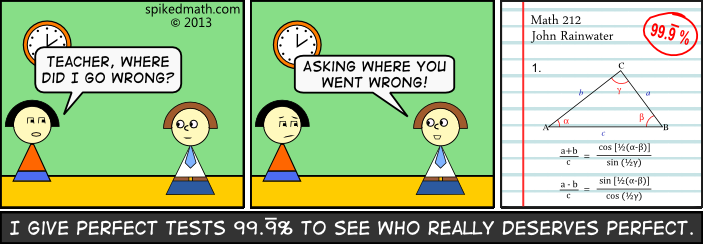
\includegraphics[width=\linewidth]{547-the-perfect-score.png}
%\includegraphics[width=0.7\linewidth]{TooManyPigeons.jpg}
\begin{center}
\tiny Mike, http://http://spikedmath.com/547.html, CC-BY-NC-2.5
%\captionof*{figure}{\hspace{3cm}Dueslagsprincippet\\ \vspace{1mm} \\ \tiny en:User:BenFrantzDale og en:User:McKay, CC-BY-SA 3.0}
\end{center}

\end{minipage}
%\hspace{2mm}
\hfill
\begin{minipage}[t]{0.32\linewidth}
\vspace{3mm}
\section*{Madandmeldelse -- DSB-kaffe}
Det ses ved første øjenkast at her er der virkelig kræset for detaljerne, udstyr til kropslig styrkelse er blandet med mentale udfordringer i symmetrisk placerede badefaciliteter og kunstnerisk udførte lysinstallationer, som spiller godt sammen med den historicistiske hovedbygning fra 1890'erne. Også for det fysiske velvære er sørget, velvidende at frost hyppigt kan forekomme i den danske sommer, så der er sørget for den nødvendige mængde kropsvarme i lokalet, og af miljøhensyn desuden sparet på udluftningen.
Endda lydbilledet er proffesionelt konstrueret, med en passende mængde af snorken, luftmadrasser der sprænges klokken tre og en decent men veliscenesat piplyd fra et ukendt sted. Gadelarmen understreger rummets urbane placering på Indre Østerbro og sirener minder jævnligt om Rigets betryggende nærhed. Hvis vinden kommer fra den rigtige retning kan der desuden bydes på skrål og gadekamp fra sportsinteresserede borgere. Som godtgørelse for denne mangel er der fremskaffet fire afdøde idrætslærere, hvis spøgelser indfører tvungen stikbold (med en flintesten) hver anden time i nattens løb og er kontraktmæssigt forpligtet til at give $-3$ til alle matematisk interesserede elever. 
De sovendes bagage indeholder løse dele, såsom brudte løfter og håb der er gået itu, så sovesalen kan ikke anbefales for børn under den aksiomatiske lavalder.

\end{minipage}
\end{minipage}
